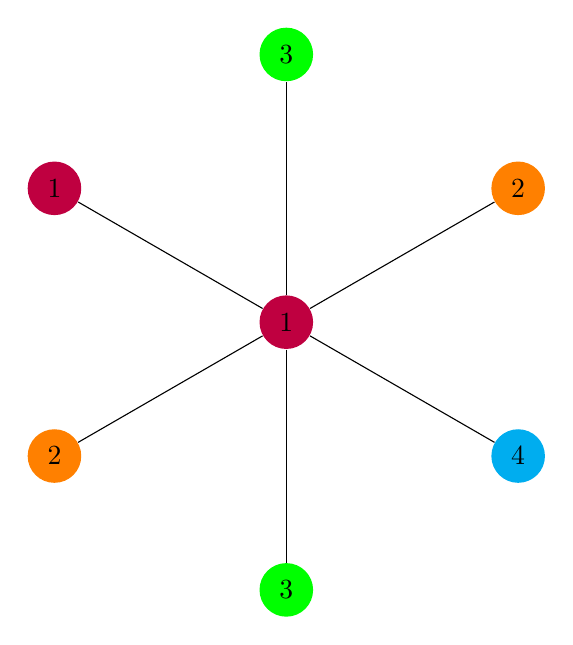
\begin{tikzpicture}[scale=2]
	
	% ---- Adjustable colors ----
	\def\centerColor{purple}
	\def\colorA{green}
	\def\colorB{orange}
	\def\colorC{cyan}
	\def\colorD{green}
	\def\colorE{orange}
	\def\colorF{purple}
	
	% ---- Positions of outer vertices (6 around a circle) ----
	\foreach \angle/\name/\col/\label in {
		90/A/\colorA/3,
		30/B/\colorB/2,
		-30/C/\colorC/4,
		-90/D/\colorD/3,
		-150/E/\colorE/2,
		150/F/\colorF/1
	}
	{
		\node[fill=\col, circle, inner sep=4pt] (v\name) at (\angle:1.7) {\label};
	}
	
	% ---- Center vertex ----
	\node[fill=\centerColor, circle, inner sep=4pt] (center) at (0,0) {1};
	
	% ---- Edges to center ----
	\foreach \name in {A,B,C,D,E,F}
	\draw (center) -- (v\name);
	
\end{tikzpicture}

